\chapter{Classification}
\label{ch:classification}

We have seen the iris data before.\marginnote{We call the variable we wish to predict a target variable, or an outcome or, in traditional machine learning terminology, a class. Hence we talk about classification, classifiers, classification trees...} We wanted to predict varieties based on measurements---but we actually did not make any predictions. We observed some potentially interesting relations between the features and the varieties, but have never constructed an actual model.

Let us create one now.

\begin{figure}[h]
    \centering
    \vspace{-0.2cm}
    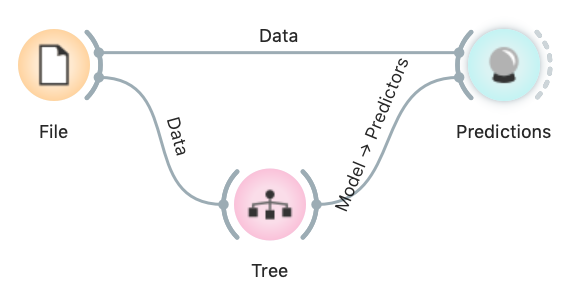
\includegraphics[scale=0.4]{predictions-workflow.png}
    \caption{Something in this workflow is conceptually wrong. Can you guess what?}
    \label{fig:spectral_preprocessing-fig2}
\end{figure}

\begin{wrapfigure}{o}{1.0\textwidth}
    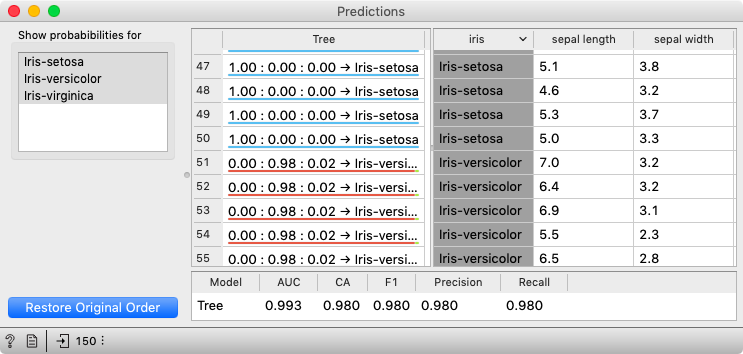
\includegraphics[scale=0.4]{predictions.png}
    \label{fig:classification-predictions}
\end{wrapfigure}

The data is fed into the \widget{Tree} widget, which infers a classification model and gives it to the Predictions widget. Note that unlike in our past workflows, in which the communication between widgets included only the data, we here have a channel that carries a predictive model.

The \widget{Predictions} widget also receives the data from the File widget. The widget uses the model to make predictions about the data and shows them in the table.

How correct are these predictions? Do we have a good model? How can we tell?

But (and even before answering these very important questions), what is a classification tree? And how does Orange create one? Is this algorithm something we should really use?

So many questions to answer!
